\documentclass[twoside]{book}

% Packages required by doxygen
\usepackage{fixltx2e}
\usepackage{calc}
\usepackage{doxygen}
\usepackage[export]{adjustbox} % also loads graphicx
\usepackage{graphicx}
\usepackage[utf8]{inputenc}
\usepackage{makeidx}
\usepackage{multicol}
\usepackage{multirow}
\PassOptionsToPackage{warn}{textcomp}
\usepackage{textcomp}
\usepackage[nointegrals]{wasysym}
\usepackage[table]{xcolor}

% NLS support packages
\usepackage[ngerman]{babel}

% Font selection
\usepackage[T1]{fontenc}
\usepackage[scaled=.90]{helvet}
\usepackage{courier}
\usepackage{amssymb}
\usepackage{sectsty}
\renewcommand{\familydefault}{\sfdefault}
\allsectionsfont{%
  \fontseries{bc}\selectfont%
  \color{darkgray}%
}
\renewcommand{\DoxyLabelFont}{%
  \fontseries{bc}\selectfont%
  \color{darkgray}%
}
\newcommand{\+}{\discretionary{\mbox{\scriptsize$\hookleftarrow$}}{}{}}

% Page & text layout
\usepackage{geometry}
\geometry{%
  a4paper,%
  top=2.5cm,%
  bottom=2.5cm,%
  left=2.5cm,%
  right=2.5cm%
}
\tolerance=750
\hfuzz=15pt
\hbadness=750
\setlength{\emergencystretch}{15pt}
\setlength{\parindent}{0cm}
\setlength{\parskip}{3ex plus 2ex minus 2ex}
\makeatletter
\renewcommand{\paragraph}{%
  \@startsection{paragraph}{4}{0ex}{-1.0ex}{1.0ex}{%
    \normalfont\normalsize\bfseries\SS@parafont%
  }%
}
\renewcommand{\subparagraph}{%
  \@startsection{subparagraph}{5}{0ex}{-1.0ex}{1.0ex}{%
    \normalfont\normalsize\bfseries\SS@subparafont%
  }%
}
\makeatother

% Headers & footers
\usepackage{fancyhdr}
\pagestyle{fancyplain}
\fancyhead[LE]{\fancyplain{}{\bfseries\thepage}}
\fancyhead[CE]{\fancyplain{}{}}
\fancyhead[RE]{\fancyplain{}{\bfseries\leftmark}}
\fancyhead[LO]{\fancyplain{}{\bfseries\rightmark}}
\fancyhead[CO]{\fancyplain{}{}}
\fancyhead[RO]{\fancyplain{}{\bfseries\thepage}}
\fancyfoot[LE]{\fancyplain{}{}}
\fancyfoot[CE]{\fancyplain{}{}}
\fancyfoot[RE]{\fancyplain{}{\bfseries\scriptsize Erzeugt von Doxygen }}
\fancyfoot[LO]{\fancyplain{}{\bfseries\scriptsize Erzeugt von Doxygen }}
\fancyfoot[CO]{\fancyplain{}{}}
\fancyfoot[RO]{\fancyplain{}{}}
\renewcommand{\footrulewidth}{0.4pt}
\renewcommand{\chaptermark}[1]{%
  \markboth{#1}{}%
}
\renewcommand{\sectionmark}[1]{%
  \markright{\thesection\ #1}%
}

% Indices & bibliography
\usepackage{natbib}
\usepackage[titles]{tocloft}
\setcounter{tocdepth}{3}
\setcounter{secnumdepth}{5}
\makeindex

% Hyperlinks (required, but should be loaded last)
\usepackage{ifpdf}
\ifpdf
  \usepackage[pdftex,pagebackref=true]{hyperref}
\else
  \usepackage[ps2pdf,pagebackref=true]{hyperref}
\fi
\hypersetup{%
  colorlinks=true,%
  linkcolor=blue,%
  citecolor=blue,%
  unicode%
}

% Custom commands
\newcommand{\clearemptydoublepage}{%
  \newpage{\pagestyle{empty}\cleardoublepage}%
}

\usepackage{caption}
\captionsetup{labelsep=space,justification=centering,font={bf},singlelinecheck=off,skip=4pt,position=top}

%===== C O N T E N T S =====

\begin{document}

% Titlepage & ToC
\hypersetup{pageanchor=false,
             bookmarksnumbered=true,
             pdfencoding=unicode
            }
\pagenumbering{alph}
\begin{titlepage}
\vspace*{7cm}
\begin{center}%
{\Large Übung Objektorientierte Programmierung \\[1ex]\large 1.\+0 }\\
\vspace*{1cm}
{\large Erzeugt von Doxygen 1.8.13}\\
\end{center}
\end{titlepage}
\clearemptydoublepage
\pagenumbering{roman}
\tableofcontents
\clearemptydoublepage
\pagenumbering{arabic}
\hypersetup{pageanchor=true}

%--- Begin generated contents ---
\chapter{Klassen-\/\+Verzeichnis}
\section{Auflistung der Klassen}
Hier folgt die Aufzählung aller Klassen, Strukturen, Varianten und Schnittstellen mit einer Kurzbeschreibung\+:\begin{DoxyCompactList}
\item\contentsline{section}{\hyperlink{class_c_counter}{C\+Counter} }{\pageref{class_c_counter}}{}
\item\contentsline{section}{\hyperlink{class_c_forward_counter}{C\+Forward\+Counter} }{\pageref{class_c_forward_counter}}{}
\item\contentsline{section}{\hyperlink{class_c_variable_counter}{C\+Variable\+Counter} }{\pageref{class_c_variable_counter}}{}
\end{DoxyCompactList}

\chapter{Datei-\/\+Verzeichnis}
\section{Auflistung der Dateien}
Hier folgt die Aufzählung aller Dateien mit einer Kurzbeschreibung\+:\begin{DoxyCompactList}
\item\contentsline{section}{C\+:/portable\+Dev\+Env\+\_\+2017/workspace2017/project/src/\hyperlink{_c_array_8hpp}{C\+Array.\+hpp} \\*Template-\/\+Klasse \hyperlink{class_c_array}{C\+Array} Erzeugt ein Array vom Typ T mit N Elementen }{\pageref{_c_array_8hpp}}{}
\item\contentsline{section}{C\+:/portable\+Dev\+Env\+\_\+2017/workspace2017/project/src/\hyperlink{_c_array_dec_8cpp}{C\+Array\+Dec.\+cpp} \\*Created on\+: 24.\+05.\+2018 Author\+: diamo }{\pageref{_c_array_dec_8cpp}}{}
\item\contentsline{section}{C\+:/portable\+Dev\+Env\+\_\+2017/workspace2017/project/src/\hyperlink{_c_array_dec_8hpp}{C\+Array\+Dec.\+hpp} \\*L\+ZW Decoder, Dictionary implementiert als Array }{\pageref{_c_array_dec_8hpp}}{}
\item\contentsline{section}{C\+:/portable\+Dev\+Env\+\_\+2017/workspace2017/project/src/\hyperlink{_c_array_enc_8cpp}{C\+Array\+Enc.\+cpp} \\*Created on\+: 24.\+05.\+2018 Author\+: diamo }{\pageref{_c_array_enc_8cpp}}{}
\item\contentsline{section}{C\+:/portable\+Dev\+Env\+\_\+2017/workspace2017/project/src/\hyperlink{_c_array_enc_8hpp}{C\+Array\+Enc.\+hpp} \\*L\+ZW Encoder, Dictionary implementiert als Array }{\pageref{_c_array_enc_8hpp}}{}
\item\contentsline{section}{C\+:/portable\+Dev\+Env\+\_\+2017/workspace2017/project/src/\hyperlink{_c_counter_8cpp}{C\+Counter.\+cpp} \\*Created on\+: 06.\+04.\+2018 Author\+: diamo }{\pageref{_c_counter_8cpp}}{}
\item\contentsline{section}{C\+:/portable\+Dev\+Env\+\_\+2017/workspace2017/project/src/\hyperlink{_c_counter_8hpp}{C\+Counter.\+hpp} \\*Created on\+: 06.\+04.\+2018 Author\+: diamo }{\pageref{_c_counter_8hpp}}{}
\item\contentsline{section}{C\+:/portable\+Dev\+Env\+\_\+2017/workspace2017/project/src/\hyperlink{_c_dec_8cpp}{C\+Dec.\+cpp} }{\pageref{_c_dec_8cpp}}{}
\item\contentsline{section}{C\+:/portable\+Dev\+Env\+\_\+2017/workspace2017/project/src/\hyperlink{_c_dec_8hpp}{C\+Dec.\+hpp} \\*Klasse \hyperlink{class_c_dec}{C\+Dec} Abstrakte Basisklasse für Decodierung }{\pageref{_c_dec_8hpp}}{}
\item\contentsline{section}{C\+:/portable\+Dev\+Env\+\_\+2017/workspace2017/project/src/\hyperlink{_c_double_hashing_8cpp}{C\+Double\+Hashing.\+cpp} \\*Created on\+: 18.\+05.\+2018 Author\+: diamo }{\pageref{_c_double_hashing_8cpp}}{}
\item\contentsline{section}{C\+:/portable\+Dev\+Env\+\_\+2017/workspace2017/project/src/\hyperlink{_c_double_hashing_8hpp}{C\+Double\+Hashing.\+hpp} \\*Klasse zum Hashen }{\pageref{_c_double_hashing_8hpp}}{}
\item\contentsline{section}{C\+:/portable\+Dev\+Env\+\_\+2017/workspace2017/project/src/\hyperlink{_c_enc_8cpp}{C\+Enc.\+cpp} }{\pageref{_c_enc_8cpp}}{}
\item\contentsline{section}{C\+:/portable\+Dev\+Env\+\_\+2017/workspace2017/project/src/\hyperlink{_c_enc_8hpp}{C\+Enc.\+hpp} \\*Klasse \hyperlink{class_c_enc}{C\+Enc} Abstrakte Basisklasse für Encodierung }{\pageref{_c_enc_8hpp}}{}
\item\contentsline{section}{C\+:/portable\+Dev\+Env\+\_\+2017/workspace2017/project/src/\hyperlink{_c_entry_8cpp}{C\+Entry.\+cpp} \\*Created on\+: 21.\+04.\+2018 Author\+: diamo }{\pageref{_c_entry_8cpp}}{}
\item\contentsline{section}{C\+:/portable\+Dev\+Env\+\_\+2017/workspace2017/project/src/\hyperlink{_c_entry_8hpp}{C\+Entry.\+hpp} \\*Enthält die Basisklasse \hyperlink{class_c_entry}{C\+Entry} Wird später von \hyperlink{class_c_knot}{C\+Knot} benötigt }{\pageref{_c_entry_8hpp}}{}
\item\contentsline{section}{C\+:/portable\+Dev\+Env\+\_\+2017/workspace2017/project/src/\hyperlink{_c_forward_counter_8cpp}{C\+Forward\+Counter.\+cpp} \\*Created on\+: 07.\+04.\+2018 Author\+: diamo }{\pageref{_c_forward_counter_8cpp}}{}
\item\contentsline{section}{C\+:/portable\+Dev\+Env\+\_\+2017/workspace2017/project/src/\hyperlink{_c_forward_counter_8hpp}{C\+Forward\+Counter.\+hpp} \\*Created on\+: 07.\+04.\+2018 Author\+: diamo }{\pageref{_c_forward_counter_8hpp}}{}
\item\contentsline{section}{C\+:/portable\+Dev\+Env\+\_\+2017/workspace2017/project/src/\hyperlink{_c_knot_8cpp}{C\+Knot.\+cpp} \\*Created on\+: 11.\+05.\+2018 Author\+: diamo }{\pageref{_c_knot_8cpp}}{}
\item\contentsline{section}{C\+:/portable\+Dev\+Env\+\_\+2017/workspace2017/project/src/\hyperlink{_c_knot_8hpp}{C\+Knot.\+hpp} \\*Enthält die Klasse \hyperlink{class_c_entry}{C\+Entry} Erbt von \hyperlink{class_c_knot}{C\+Knot} }{\pageref{_c_knot_8hpp}}{}
\item\contentsline{section}{C\+:/portable\+Dev\+Env\+\_\+2017/workspace2017/project/src/\hyperlink{_c_l_z_w_8cpp}{C\+L\+Z\+W.\+cpp} }{\pageref{_c_l_z_w_8cpp}}{}
\item\contentsline{section}{C\+:/portable\+Dev\+Env\+\_\+2017/workspace2017/project/src/\hyperlink{_c_l_z_w_8hpp}{C\+L\+Z\+W.\+hpp} \\*\hyperlink{_c_l_z_w_8hpp}{C\+L\+Z\+W.\+hpp} Basisklasse für L\+ZW Encoder und Decoder }{\pageref{_c_l_z_w_8hpp}}{}
\item\contentsline{section}{C\+:/portable\+Dev\+Env\+\_\+2017/workspace2017/project/src/\hyperlink{_c_trie_dec_8cpp}{C\+Trie\+Dec.\+cpp} \\*Created on\+: 29.\+05.\+2018 Author\+: diamo }{\pageref{_c_trie_dec_8cpp}}{}
\item\contentsline{section}{C\+:/portable\+Dev\+Env\+\_\+2017/workspace2017/project/src/\hyperlink{_c_trie_dec_8hpp}{C\+Trie\+Dec.\+hpp} \\*L\+ZW Decoder, Dictionary implementiert als Trie }{\pageref{_c_trie_dec_8hpp}}{}
\item\contentsline{section}{C\+:/portable\+Dev\+Env\+\_\+2017/workspace2017/project/src/\hyperlink{_c_trie_enc_8cpp}{C\+Trie\+Enc.\+cpp} \\*Created on\+: 29.\+05.\+2018 Author\+: diamo }{\pageref{_c_trie_enc_8cpp}}{}
\item\contentsline{section}{C\+:/portable\+Dev\+Env\+\_\+2017/workspace2017/project/src/\hyperlink{_c_trie_enc_8hpp}{C\+Trie\+Enc.\+hpp} \\*L\+ZW Encoder, Dictionary implementiert als Trie }{\pageref{_c_trie_enc_8hpp}}{}
\item\contentsline{section}{C\+:/portable\+Dev\+Env\+\_\+2017/workspace2017/project/src/\hyperlink{main_praktikum_8cpp}{main\+Praktikum.\+cpp} }{\pageref{main_praktikum_8cpp}}{}
\item\contentsline{section}{C\+:/portable\+Dev\+Env\+\_\+2017/workspace2017/project/src/\hyperlink{_x_out_of_bounds_8cpp}{X\+Out\+Of\+Bounds.\+cpp} \\*Created on\+: 10.\+05.\+2018 Author\+: diamo }{\pageref{_x_out_of_bounds_8cpp}}{}
\item\contentsline{section}{C\+:/portable\+Dev\+Env\+\_\+2017/workspace2017/project/src/\hyperlink{_x_out_of_bounds_8hpp}{X\+Out\+Of\+Bounds.\+hpp} \\*Enthält die Klasse \hyperlink{class_x_out_of_bounds}{X\+Out\+Of\+Bounds} Es handelt sich hierbei um eine Klasse die Ausnahmeobjekte erstellt }{\pageref{_x_out_of_bounds_8hpp}}{}
\end{DoxyCompactList}

\chapter{Klassen-\/\+Dokumentation}
\hypertarget{class_another_test}{}\section{Another\+Test Klassenreferenz}
\label{class_another_test}\index{Another\+Test@{Another\+Test}}


Zusammengehörigkeiten von Another\+Test\+:\nopagebreak
\begin{figure}[H]
\begin{center}
\leavevmode
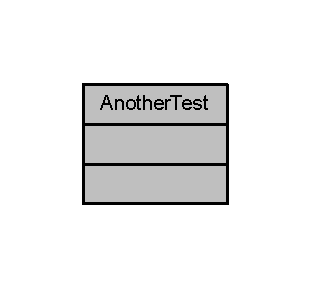
\includegraphics[width=149pt]{class_another_test__coll__graph}
\end{center}
\end{figure}


Die Dokumentation für diese Klasse wurde erzeugt aufgrund der Datei\+:\begin{DoxyCompactItemize}
\item 
C\+:/portable\+Dev\+Env\+\_\+2017/workspace2017/\+Blatt1\+\_\+\+Doxygen/src/\hyperlink{_blatt1___doxygen_8cpp}{Blatt1\+\_\+\+Doxygen.\+cpp}\end{DoxyCompactItemize}

\hypertarget{class_q_tstyle___test}{}\section{Q\+Tstyle\+\_\+\+Test Klassenreferenz}
\label{class_q_tstyle___test}\index{Q\+Tstyle\+\_\+\+Test@{Q\+Tstyle\+\_\+\+Test}}


A test class. This is a brief description, if length is only one line.  




Zusammengehörigkeiten von Q\+Tstyle\+\_\+\+Test\+:\nopagebreak
\begin{figure}[H]
\begin{center}
\leavevmode
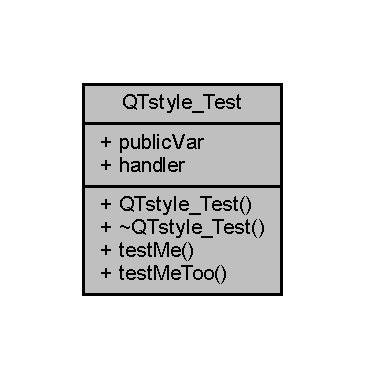
\includegraphics[width=175pt]{class_q_tstyle___test__coll__graph}
\end{center}
\end{figure}
\subsection*{Öffentliche Methoden}
\begin{DoxyCompactItemize}
\item 
\hyperlink{class_q_tstyle___test_a14a296ea4e2ad446712f2310bec60766}{Q\+Tstyle\+\_\+\+Test} ()
\begin{DoxyCompactList}\small\item\em A constructor. \end{DoxyCompactList}\item 
virtual \hyperlink{class_q_tstyle___test_a0ad2e372fe09f34fce46b570b297ae79}{$\sim$\+Q\+Tstyle\+\_\+\+Test} ()
\begin{DoxyCompactList}\small\item\em A destructor. \end{DoxyCompactList}\item 
int \hyperlink{class_q_tstyle___test_a8840748753118dd468e8368a28e49c62}{test\+Me} (int a, const char $\ast$s)
\begin{DoxyCompactList}\small\item\em A normal member taking two arguments and returning an integer value. \end{DoxyCompactList}\item 
virtual void \hyperlink{class_q_tstyle___test_ad5b201f097a720d44bf976c2f27efbda}{test\+Me\+Too} (char c1, char c2)=0
\begin{DoxyCompactList}\small\item\em A pure virtual member. \end{DoxyCompactList}\end{DoxyCompactItemize}
\subsection*{Öffentliche Attribute}
\begin{DoxyCompactItemize}
\item 
int \hyperlink{class_q_tstyle___test_aabf7b2e9ed83ea44aca4d213baae06d3}{public\+Var}
\begin{DoxyCompactList}\small\item\em A public variable. \end{DoxyCompactList}\item 
int($\ast$ \hyperlink{class_q_tstyle___test_a79dd4e5498f09057775a819d911349e2}{handler} )(int a, int b)
\begin{DoxyCompactList}\small\item\em A function variable. \end{DoxyCompactList}\end{DoxyCompactItemize}


\subsection{Ausführliche Beschreibung}
A test class. This is a brief description, if length is only one line. 

A more elaborate class description. 

\subsection{Beschreibung der Konstruktoren und Destruktoren}
\mbox{\Hypertarget{class_q_tstyle___test_a14a296ea4e2ad446712f2310bec60766}\label{class_q_tstyle___test_a14a296ea4e2ad446712f2310bec60766}} 
\index{Q\+Tstyle\+\_\+\+Test@{Q\+Tstyle\+\_\+\+Test}!Q\+Tstyle\+\_\+\+Test@{Q\+Tstyle\+\_\+\+Test}}
\index{Q\+Tstyle\+\_\+\+Test@{Q\+Tstyle\+\_\+\+Test}!Q\+Tstyle\+\_\+\+Test@{Q\+Tstyle\+\_\+\+Test}}
\subsubsection{\texorpdfstring{Q\+Tstyle\+\_\+\+Test()}{QTstyle\_Test()}}
{\footnotesize\ttfamily Q\+Tstyle\+\_\+\+Test\+::\+Q\+Tstyle\+\_\+\+Test (\begin{DoxyParamCaption}{ }\end{DoxyParamCaption})}



A constructor. 

A more elaborate description of the constructor. \mbox{\Hypertarget{class_q_tstyle___test_a0ad2e372fe09f34fce46b570b297ae79}\label{class_q_tstyle___test_a0ad2e372fe09f34fce46b570b297ae79}} 
\index{Q\+Tstyle\+\_\+\+Test@{Q\+Tstyle\+\_\+\+Test}!````~Q\+Tstyle\+\_\+\+Test@{$\sim$\+Q\+Tstyle\+\_\+\+Test}}
\index{````~Q\+Tstyle\+\_\+\+Test@{$\sim$\+Q\+Tstyle\+\_\+\+Test}!Q\+Tstyle\+\_\+\+Test@{Q\+Tstyle\+\_\+\+Test}}
\subsubsection{\texorpdfstring{$\sim$\+Q\+Tstyle\+\_\+\+Test()}{~QTstyle\_Test()}}
{\footnotesize\ttfamily virtual Q\+Tstyle\+\_\+\+Test\+::$\sim$\+Q\+Tstyle\+\_\+\+Test (\begin{DoxyParamCaption}{ }\end{DoxyParamCaption})\hspace{0.3cm}{\ttfamily [virtual]}}



A destructor. 

A more elaborate description of the destructor. 

\subsection{Dokumentation der Elementfunktionen}
\mbox{\Hypertarget{class_q_tstyle___test_a8840748753118dd468e8368a28e49c62}\label{class_q_tstyle___test_a8840748753118dd468e8368a28e49c62}} 
\index{Q\+Tstyle\+\_\+\+Test@{Q\+Tstyle\+\_\+\+Test}!test\+Me@{test\+Me}}
\index{test\+Me@{test\+Me}!Q\+Tstyle\+\_\+\+Test@{Q\+Tstyle\+\_\+\+Test}}
\subsubsection{\texorpdfstring{test\+Me()}{testMe()}}
{\footnotesize\ttfamily int Q\+Tstyle\+\_\+\+Test\+::test\+Me (\begin{DoxyParamCaption}\item[{int}]{a,  }\item[{const char $\ast$}]{s }\end{DoxyParamCaption})}



A normal member taking two arguments and returning an integer value. 


\begin{DoxyParams}{Parameter}
{\em a} & an integer argument. \\
\hline
{\em s} & a constant character pointer. \\
\hline
\end{DoxyParams}
\begin{DoxyReturn}{Rückgabe}
The test results 
\end{DoxyReturn}
\begin{DoxySeeAlso}{Siehe auch}
\hyperlink{class_q_tstyle___test_a14a296ea4e2ad446712f2310bec60766}{Q\+Tstyle\+\_\+\+Test()}, \hyperlink{class_q_tstyle___test_a0ad2e372fe09f34fce46b570b297ae79}{$\sim$\+Q\+Tstyle\+\_\+\+Test()}, \hyperlink{class_q_tstyle___test_ad5b201f097a720d44bf976c2f27efbda}{test\+Me\+Too()} and \hyperlink{class_q_tstyle___test_aabf7b2e9ed83ea44aca4d213baae06d3}{public\+Var()} 
\end{DoxySeeAlso}
\mbox{\Hypertarget{class_q_tstyle___test_ad5b201f097a720d44bf976c2f27efbda}\label{class_q_tstyle___test_ad5b201f097a720d44bf976c2f27efbda}} 
\index{Q\+Tstyle\+\_\+\+Test@{Q\+Tstyle\+\_\+\+Test}!test\+Me\+Too@{test\+Me\+Too}}
\index{test\+Me\+Too@{test\+Me\+Too}!Q\+Tstyle\+\_\+\+Test@{Q\+Tstyle\+\_\+\+Test}}
\subsubsection{\texorpdfstring{test\+Me\+Too()}{testMeToo()}}
{\footnotesize\ttfamily virtual void Q\+Tstyle\+\_\+\+Test\+::test\+Me\+Too (\begin{DoxyParamCaption}\item[{char}]{c1,  }\item[{char}]{c2 }\end{DoxyParamCaption})\hspace{0.3cm}{\ttfamily [pure virtual]}}



A pure virtual member. 

\begin{DoxySeeAlso}{Siehe auch}
\hyperlink{class_q_tstyle___test_a8840748753118dd468e8368a28e49c62}{test\+Me()} 
\end{DoxySeeAlso}

\begin{DoxyParams}{Parameter}
{\em c1} & the first argument. \\
\hline
{\em c2} & the second argument. \\
\hline
\end{DoxyParams}


\subsection{Dokumentation der Datenelemente}
\mbox{\Hypertarget{class_q_tstyle___test_a79dd4e5498f09057775a819d911349e2}\label{class_q_tstyle___test_a79dd4e5498f09057775a819d911349e2}} 
\index{Q\+Tstyle\+\_\+\+Test@{Q\+Tstyle\+\_\+\+Test}!handler@{handler}}
\index{handler@{handler}!Q\+Tstyle\+\_\+\+Test@{Q\+Tstyle\+\_\+\+Test}}
\subsubsection{\texorpdfstring{handler}{handler}}
{\footnotesize\ttfamily int($\ast$ Q\+Tstyle\+\_\+\+Test\+::handler) (int a, int b)}



A function variable. 

Details. \mbox{\Hypertarget{class_q_tstyle___test_aabf7b2e9ed83ea44aca4d213baae06d3}\label{class_q_tstyle___test_aabf7b2e9ed83ea44aca4d213baae06d3}} 
\index{Q\+Tstyle\+\_\+\+Test@{Q\+Tstyle\+\_\+\+Test}!public\+Var@{public\+Var}}
\index{public\+Var@{public\+Var}!Q\+Tstyle\+\_\+\+Test@{Q\+Tstyle\+\_\+\+Test}}
\subsubsection{\texorpdfstring{public\+Var}{publicVar}}
{\footnotesize\ttfamily int Q\+Tstyle\+\_\+\+Test\+::public\+Var}



A public variable. 

Details. 

Die Dokumentation für diese Klasse wurde erzeugt aufgrund der Datei\+:\begin{DoxyCompactItemize}
\item 
C\+:/portable\+Dev\+Env\+\_\+2017/workspace2017/\+Blatt1\+\_\+\+Doxygen/src/\hyperlink{_blatt1___doxygen_8cpp}{Blatt1\+\_\+\+Doxygen.\+cpp}\end{DoxyCompactItemize}

\hypertarget{class_test}{}\section{Test Klassenreferenz}
\label{class_test}\index{Test@{Test}}


Short documentation of \hyperlink{class_another_test}{Another\+Test}, located not directly in front of the class definition.  




Zusammengehörigkeiten von Test\+:\nopagebreak
\begin{figure}[H]
\begin{center}
\leavevmode
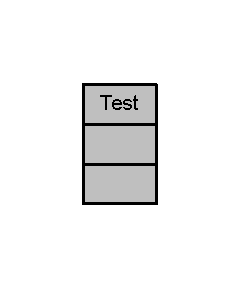
\includegraphics[width=115pt]{class_test__coll__graph}
\end{center}
\end{figure}


\subsection{Ausführliche Beschreibung}
Short documentation of \hyperlink{class_another_test}{Another\+Test}, located not directly in front of the class definition. 

This documentation is not located directly in front of the class definition. This is allowed, but the following structural commands have to be used as required, starting with a backslash symbol.

struct to document a C-\/struct. union to document a union. enum to document an enumeration type. fn to document a function. var to document a variable or typedef or enum value. def to document a define. typedef to document a type definition. file to document a file. namespace to document a namespace. package to document a Java package. interface to document an I\+DL interface.

see \href{https://www.stack.nl/~dimitri/doxygen/manual/docblocks.html}{\tt https\+://www.\+stack.\+nl/$\sim$dimitri/doxygen/manual/docblocks.\+html} 

Die Dokumentation für diese Klasse wurde erzeugt aufgrund der Datei\+:\begin{DoxyCompactItemize}
\item 
C\+:/portable\+Dev\+Env\+\_\+2017/workspace2017/\+Blatt1\+\_\+\+Doxygen/src/\hyperlink{_blatt1___doxygen_8cpp}{Blatt1\+\_\+\+Doxygen.\+cpp}\end{DoxyCompactItemize}

\chapter{Datei-\/\+Dokumentation}
\hypertarget{_blatt1___doxygen_8cpp}{}\section{C\+:/portable\+Dev\+Env\+\_\+2017/workspace2017/\+Blatt1\+\_\+\+Doxygen/src/\+Blatt1\+\_\+\+Doxygen.cpp-\/\+Dateireferenz}
\label{_blatt1___doxygen_8cpp}\index{C\+:/portable\+Dev\+Env\+\_\+2017/workspace2017/\+Blatt1\+\_\+\+Doxygen/src/\+Blatt1\+\_\+\+Doxygen.\+cpp@{C\+:/portable\+Dev\+Env\+\_\+2017/workspace2017/\+Blatt1\+\_\+\+Doxygen/src/\+Blatt1\+\_\+\+Doxygen.\+cpp}}


A short example (only) for documentation with doxygen.  


{\ttfamily \#include $<$iostream$>$}\newline
Include-\/\+Abhängigkeitsdiagramm für Blatt1\+\_\+\+Doxygen.\+cpp\+:
\nopagebreak
\begin{figure}[H]
\begin{center}
\leavevmode
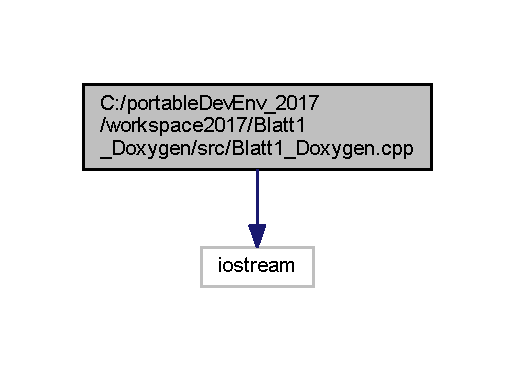
\includegraphics[width=247pt]{_blatt1___doxygen_8cpp__incl}
\end{center}
\end{figure}
\subsection*{Klassen}
\begin{DoxyCompactItemize}
\item 
class \hyperlink{class_q_tstyle___test}{Q\+Tstyle\+\_\+\+Test}
\begin{DoxyCompactList}\small\item\em A test class. This is a brief description, if length is only one line. \end{DoxyCompactList}\item 
class \hyperlink{class_another_test}{Another\+Test}
\end{DoxyCompactItemize}
\subsection*{Funktionen}
\begin{DoxyCompactItemize}
\item 
int \hyperlink{_blatt1___doxygen_8cpp_ae66f6b31b5ad750f1fe042a706a4e3d4}{main} ()
\end{DoxyCompactItemize}


\subsection{Ausführliche Beschreibung}
A short example (only) for documentation with doxygen. 

From eclipse execute the program doxygen by the following steps\+:
\begin{DoxyEnumerate}
\item Open source-\/file with doxygen-\/compatible comments (e.\+g. \hyperlink{_blatt1___doxygen_8cpp}{Blatt1\+\_\+\+Doxygen.\+cpp}) in the editor and click into the editor window.
\item Run-\/$>$ external tools -\/$>$ \char`\"{}\+Doxygen für alle Projekte (aus Blatt1\+\_\+\+Doxygen)\char`\"{} In case of other projects the file \char`\"{}\+Blatt1\+\_\+\+Doxygen/doxy/\+Doxygen für alle Projekte (aus Blatt1\+\_\+\+Doxygen).\+launch\char`\"{} is required and therefore project Blatt1\+\_\+\+Doxygen must be opened as well. 3a. H\+T\+M\+L-\/output\+: Double-\/click doxy/html/index.\+html 3b. La\+Te\+X-\/output as pdf\+: Run-\/$>$ external tools-\/$>$ \char`\"{}\+Preview Document in sumatra P\+D\+F\char`\"{} opens external viewer Sumatra\+P\+DF or Double-\/click doxy/latex/refman.\+pdf opens the internal viewer pdf4\+Eclipse This seems to work only, after doxy\textbackslash{}latex\textbackslash{}make.\+bat has been run once. Double-\/click on make.\+bat in this case.
\end{DoxyEnumerate}

See also Z\+\_\+\+Doxygen.\+pdf in Stud\+IP and the Link \href{https://www.stack.nl/~dimitri/doxygen/manual/docblocks.html}{\tt https\+://www.\+stack.\+nl/$\sim$dimitri/doxygen/manual/docblocks.\+html} In doxygen there is a C++ notation (used in this lecture) and a Java notation.

The first line starting with command file containing the file name is required for documenting e.\+g. global functions. The second line starting with command brief contains the one-\/line-\/short-\/description, ending with a blank line. The following lines contain the long version of the documentation.

This program just contains a very simple class to demonstrate doxygen comments. For member functions the documentation can be placed directly above the declaration (in the header file $\ast$.hpp) of directly above the definition (in the source file $\ast$.cpp).

The comments containing documentation in doxygen style are usually placed immediately in front of a declaration or definition of classes, memberfunctions, membervariables etc., often the brief description in front of the declaration and the long documentation in front of the definition. The documentation of all classes etc. could be collected at the front of a file, but in this case structural commands have to be used, see below.

For documentation of global objects (functions, typedefs, enums, macros etc.) the file-\/command must also be used. For documentation of members of a class that class must also be documented.

Only for member functions and member variables the documentation may be located directly behind the respective member. All other documentation is located immediately ahead of the entity, of in arbitrary position in combination with structural commands.

Doxygen knows quite a few equivalent notations, but be aware of the subtle differences. 

\subsection{Dokumentation der Funktionen}
\mbox{\Hypertarget{_blatt1___doxygen_8cpp_ae66f6b31b5ad750f1fe042a706a4e3d4}\label{_blatt1___doxygen_8cpp_ae66f6b31b5ad750f1fe042a706a4e3d4}} 
\index{Blatt1\+\_\+\+Doxygen.\+cpp@{Blatt1\+\_\+\+Doxygen.\+cpp}!main@{main}}
\index{main@{main}!Blatt1\+\_\+\+Doxygen.\+cpp@{Blatt1\+\_\+\+Doxygen.\+cpp}}
\subsubsection{\texorpdfstring{main()}{main()}}
{\footnotesize\ttfamily int main (\begin{DoxyParamCaption}{ }\end{DoxyParamCaption})}

$<$ Short description of var1

$<$ Long description of var2 using multiple lines

$<$ Long description of var3 
%--- End generated contents ---

% Index
\backmatter
\newpage
\phantomsection
\clearemptydoublepage
\addcontentsline{toc}{chapter}{Index}
\printindex

\end{document}
